\documentclass[12pt]{report}

\usepackage[ngerman]{babel}
\usepackage[utf8]{inputenc}
%\usepackage[familydefault,light]{Chivo}
\usepackage[T1]{fontenc}
\usepackage{csquotes}
\usepackage{graphicx}
\usepackage[onehalfspacing]{setspace}
\usepackage[a4paper, left=2.5cm, right=2.5cm, top=2.5cm, bottom=2.5cm]{geometry}
\usepackage{tikz}
\usepackage{aeguill}
\usepackage{scalefnt}
\usepackage{url}
\usepackage{hyperref}
\usepackage[figure]{hypcap}
\usepackage{fancyhdr}
\usepackage{verbatim}
\usepackage[printonlyused, nohyperlinks]{acronym}
\usepackage[extendedfeature=title]{scrextend}


%\bibliographystyle{abbrvdin}
\title{Vorhersage von Hotlinenutzung mit sensiblen Anrufszenarien}
\subtitle{Analyse der Telefonhotline zu Gewalt gegen Frauen in Brasilien 'Ligue 180'}
\author{Chiara Vogt Melian}
\date{\today}
\newtheorem{causal_model_definition}{Definition}[subsubsection] %TODO Theorem/Definition 

\begin{document}
	\maketitle
	\thispagestyle{empty}
	\newpage
	\pagenumbering{Roman}
	\setcounter{page}{2}
	\begin{spacing}{1}
		\chapter*{Abstract} 
		\addcontentsline{toc}{section}{Abstract}
		\renewcommand{\abstract}{}
		\abstract
	\end{spacing}
	%\newpage
	\begin{spacing}{1}
		\chapter*{Anmerkungen} 
		\addcontentsline{toc}{section}{Anmerkungen}
		%\renewcommand{\anmerkungname}{}	
		Die wörtlichen Zitate auf Englisch wurden aus Gründen der Nachvollziehbarkeit mit dem Übersetzer deepl.com übersetzt. 	
	\end{spacing}
	\newpage
	\begin{spacing}{1}
		
		\tableofcontents
	\end{spacing}
	\newpage
	
	\begin{spacing}{1}
		\chapter*{Abbildungsverzeichnis} 
		\addcontentsline{toc}{section}{Abbildungsverzeichnis}
		\renewcommand{\listfigurename}{}
		\listoffigures
	\end{spacing}
	\newpage
	\chapter*{Tabellenverzeichnis} 
	\addcontentsline{toc}{section}{Tabellenverzeichnis} 
	\renewcommand{\listtablename}{}
	\listoftables % Tabellenverzeichnis
	\footnote{Alle Tabellen wurden eigenständig erstellt, siehe \emph{R}-Code}  %TODO Anmerkung zu Tabellen überarbeiten
	\newpage
	\chapter*{Symbolverzeichnis} 
	\addcontentsline{toc}{section}{Symbolverzeichnis} %TODO Überarbeitung Symbolverzeichnis
	%Sortieren nach Auftreten im Text
	\begin{table}[h] \begin{center} \begin{tabular}{|lll|} \hline 
				& \textbf{Symbol} & \textbf{Bedeutung} \\ \hline \hline
				& $H_0 \colon$ &Nullhypothese\\ 
				& $H_1 \colon$ &Alternativhypothese\\
				& $\mathbf{I}_n\colon$ &Einheitsmatrix der Dimension $n$\\
				& $k$ &Anzahl der unabhängigen Variablen\\
				& $L(\cdot)$ &Plausibilitätsfunktion bzw. Likelihood-Funktion\\ 
				& $\ell(\cdot)$ & logarithmische Plausibilitätsfunktion bzw. log-Likelihood-Funktion\\ 
				& $n\colon$& Stichprobenumfang\\
				& $p$ &Anzahl der Regressionsparameter\\
				& $R^2\colon$ & Bestimmtheitsmaß\\ 
				& $\overline{R}^2\colon$ & adjustiertes Bestimmtheitsmaß\\ 
				& $\mathbf{X}\colon$& Versuchsplanmatrix \\ 
				& $\beta_1,\beta_2, \ldots, \beta_k\colon$& unbekannte Regressionsparameter\\ 
				& $ G_\Phi(\vartheta)$& Gütefunktion\\ 
				\hline
	\end{tabular} \end{center} \end{table}
	\newpage
	\chapter*{Abkürzungsverzeichnis} 
	\addcontentsline{toc}{section}{Abkürzungsverzeichnis} %TODO Abkürzungsverzeichnis überarbeitet?
	\begin{spacing}{0.1}
		\begin{acronym}		
			\acro{dag}[DAG]{gerichteter azyklischer Graph}
			\acro{kg}[KG]{Knowledge Graph}		
			\acro{owl}[OWL]{Web Ontology Language}
			\acro{rdf}[RDF]{Resource Description Framework}
			\acro{uri}[URI]{Universal Resource Identifier}
			\acro{xml}[XML]{eXtensible Markup Language}
		\end{acronym}
	\end{spacing}	
	\newpage
	\clearpage
	\pagenumbering{arabic}
	\setcounter{page}{1} 
	\newpage
	\pagestyle{fancy}
	\fancyhead[L]{Chiara Vogt Melian}
	\fancyhead[R]{\textbf{Zeitreihenanalyse der Telefonhotline 'Ligue 180'}}
	
	\renewcommand{\headrulewidth}{0.1 pt}
	\renewcommand{\footrulewidth}{0 pt}
	
	\chapter{Einleitung}
	
	\section{Potenzial der Prediction Models für} %TODO Wofür steht diese Arbeit besipielhaft?
	\section{Fragestellung}
	Im nächsten Abschnitt wird erläutert, welche Schwerpunkte die Analyse des Datensatzes \textit{Ligue 180} beinhaltet. In Form von Forschungsfragen und Hypothesen leiten diese inhaltlich durch die Arbeit. 
	\section{Gliederung der Arbeit}
	\subsection{Forecasting der Anrufquote}
	Die Arbeit wird drei Themenbereiche abdecken und die Analyse des Datensatzes dabei jeweils um eine Komponente erweitern. Der erste Teil der Analyse betrachtet die Menge der Anrufe, und hat zum Ziel vorherzusagen, wann wie viele Anrufe getätigt werden, um eine ausreichende Deckung der Hotline sicherzustellen. Dafür werden die Methoden der Time Series Analysis und des Forecasting genutzt. \\
	\subsection{Clusteranalyse der Nutzer:innengruppen}
	\subsection{Raumcluster und Zusammenhänge}
	\chapter{Grundlagen} 
	\section{Verwandte Arbeiten (Influential Research)} 
	%TODO die Frau mit dem Github-Projekt und der Datenanalyse da drin
	\section{Erwartete Ergebnisse}
	\chapter{Vorbereitung der Daten}
	\section{Der 'Ligue 180'-Datensatz}
	%TODO herausfinden, ob der Datensatz nur die Anzeigen speichert 
	%TODO noch was zu der Verteilung sagen im Vergleich zu allen Anrufen
	%TODO und zu der Entwicklung des Datensatzes
	
	Die Daten sind aus einem durch die brasilianische Regierung zur Verfügung gestellten Datensatz des Ministeriums für Menschen- und Bürgerrecht\footnote{Übersetzung: Ministério dos Direitos Humanos e da Cidadania, URL: \url{https://www.gov.br/mdh/pt-br}, zuletzt aufgerufen am: 30.09.2024, 15:01 Uhr}. Der Datensatz beinhaltet die Meldungen von Gewalt gegen Frauen,  die bei der Hotline 'Ligue 180' eingegangen sind. Er besteht aus 17 einzelnen Datensätzen und erstreckt sich über die Jahre 2014 bis zum ersten Halbjahr 2024\footnote{Quelle der Daten: \url{https://www.gov.br/mdh/pt-br/acesso-a-informacao/dados-abertos/ligue180} und /url{https://dados.gov.br/dados/conjuntos-dados/central-de-atendimento-a-mulher--ligue-180} (aufgerufen am 02.10.2024, 07:08 Uhr).}. %TODO: das ist keine Fußnote sondern muss in die Quellen!--beides\\
	%TODO Relatorio lesen und als Quelle einfügen, wichtige Punkte rausarbeiten
	Insgesamt enthalten alle Datensätze zusammen 2.406.112 Einträge; ab 2020 hat der Datensatz die gleiche Struktur und ergibt 1.681.161 Einträge mit 62 Kategorien. Diese Menge an Daten ist selbst bei einer großen Anzahl ungültiger Werte ausreichend für die maschinelle Verarbeitung.\\
	Durch das brasilianische Gesetz des Zugangs zu Informationen 12.527\footnote{\url{http://www.planalto.gov.br/ccivil_03/_ato2011-2014/2011/lei/l12527.htm} %TODO als Quelle
	(aufgerufen am 02.10.2024, 08:41 Uhr)} werden Leitlinien festgesetzt, die den Zugang zu staatlich erhobenen Daten ermöglichen. Dadurch kann auf den Datensatz 'Central de Atendimento à Mulher – Ligue 180' über das \textit{Portal der offenen Daten} zugegriffen werden\footnote{\url{https://dados.gov.br/dados/conjuntos-dados/central-de-atendimento-a-mulher--ligue-180} (aufgerufen am 02.10.2024, 08:48 Uhr)}.
	\section{Datenauswahl}
	Eine anfängliche Durchsicht der Einträge zeigt, dass nicht alle für eine Verarbeitung geeignet sind. Die Rohdaten haben eine Menge von 2.406.097 Einträgen, darin befinden sich ab 2020 Daten mit gleichem Key \textit{hash}\footnote{Für das erste Semester 2020 heißt der Key \textit{hash\_par\_vitima\_suspeito}.} und gleichem Timestamp. Diese wurden augenscheinlich mehrmals aufgenommen, um mehrere Tatschwerpunkte festzuhalten. In Tabelle \ref{tab:gleicher-hash} kann beispielhaft nachvollzogen werden, welche Unterschiede in Werten mit dem gleichen \textit{hash} zu finden sind. 
	Nach der Eliminierung dieser Duplikate verbleiben 1.069.407 Datenpunkte.\\	
	\begin {table}[ht] %TODO Tabelle hübsch machen
		\caption {hash: d2d9664e8a2fb21d0a441753b3532b3a (Vorkommen: 69)} \label{tab:gleicher-hash} 
		\centering
		\small
		\begin{tabular}{|l|l|}
		\hline
		'Profissão\_do\_suspeito' & 'CONSELHEIRO TUTELAR'\\
		\hline
		'violacao' & 'INTEGRIDADE>PATRIMONIAL>INDIVIDUAL'\\
		~ & 'INTEGRIDADE>FÍSICA>MAUS TRATOS'\\
		~ & 'INTEGRIDADE>PSÍQUICA>AMEAÇA ou COAÇÃO'\\
		~ & 'INTEGRIDADE>PSÍQUICA>CONSTRANGIMENTO' \\
		\hline
		'Motivação' & 'PARA FINS DE EXPLORAÇÃO DO TRABALHO.COMÉRCIO/ INDÚSTRIA'\\
		~ & 'EM RAZÃO DE CONDIÇÕES FÍSICAS, SENSORIAIS, INTELECTUAIS OU MENTAIS'\\
		~ & 'POR CONFLITO AGRÁRIO.QUILOMBOLAS'\\
		~ & ... \\
		~ & 'PARA FINS DE EXPLORAÇÃO SEXUAL' 'EM RAZÃO DA RELAÇÃO DE ENSINO'\\
		~ & 'POR CONFLITO AGRÁRIO.PESCA'\\
		~ & 'COM HUMILHAÇÃO' 'EM RAZÃO DA PROFISSÃO'\\
		~ & ...\\
		~ & 'DA COABITAÇÃO/ CONVIVÊNCIA FAMILIAR/ RELAÇÃO AFETIVA'\\
		~ & 'FOI PRATICADO POR DUAS OU MAIS PESSOAS'\\
		~ & 'PARA FINS DE EXPLORAÇÃO DO TRABALHO.DOMÉSTICO'\\
		~ & 'PARA FINS DE REMOÇÃO DE ÓRGÃOS/ TRÁFICO DE ÓRGÃOS'\\
		~ & 'EM PÚBLICO OU POR MEIO QUE FACILITE A DIVULGAÇÃO/ NO ÂMBITO DA INTERNET'\\
		~ & 'POR CONDUTAS EXCESSIVAS/ DESNECESSÁRIAS/ DESACONSELHADAS'\\
		~ & 'NA FORMA DE AUXÍLIO/INSTIGAÇÃO/INDUZIMENTO/INCITAÇÃO'\\
		~ & 'PARA FINS DE EXPLORAÇÃO DO TRABALHO.INFORMAL'\\
		~ & 'FALTA DE ACESSIBILIDADE.NOS MEIOS DE TRANSPORTE'\\
		~ & 'EM DESCUMPRIMENTO DE MEDIDA PROTETIVA' 'EM RAZÃO DO SEXO BIOLÓGICO'\\
		~ & 'RESULTANDO EM LESÃO SEGUIDA DE MORTE' 'RESULTANDO EM LESÃO LEVE'\\
		~ & 'NA FORMA CULPOSA' 'POR VIOLÊNCIA INSTITUCIONAL' 'COM FINS CORRETIVOS'\\
		~ & 'RESULTANDO EM LESÃO GRAVE'\\
		~ & 'DO AGRESSOR POSSUIR INFLUÊNCIA JUNTO ÀS AUTORIDADES LOCAIS'\\
		~ & 'NA RELAÇÃO FAMILIAR' 'EM RAZÃO DE CONFLITO DE IDEIAS'\\
		~ & 'EM RAZÃO DA RELIGIÃO' 'EM RAZÃO DE RAÇA/COR'\\
		~ & 'PARA FINS DE EXPLORAÇÃO DO TRABALHO.OUTROS'\\
		~ & 'PARA OBTENÇÃO DE BENEFÍCIO FINANCEIRO/ GANÂNCIA' 'EM RAZÃO DA IDADE'\\
		~ & 'POR CRIME AMBIENTAL.COM FINS DE EXTRATIVISMO.MINERAL'\\
		~ & 'POR CRIME AMBIENTAL.PESCA'\\
		~ & 'RESULTANDO EM UMA DEFICIÊNCIA EM RAZÃO DA VIOLÊNCIA'\\
		~ & 'EM RAZÃO DE ORIENTAÇÃO SEXUAL/ IDEOLOGIA DE GÊNERO'\\
		~ & 'POR CRIME AMBIENTAL.DE CAÇA' 'PARA FINS DE EXPLORAÇÃO DO TRABALHO.RURAL'\\
		~ & 'COM RESULTADO MORTE' 'EM RAZÃO DA ORIGEM'\\
		~ & 'POR MOTIVO VIL, TORPE, INSIDIOSO, CRUEL, À TRAIÇÃO, OU POR DINHEIRO'\\
		~ & 'EM RAZÃO DE SER MULHER' 'COM VÍTIMA EM SITUAÇÃO DE RUA'\\
		~ & 'FALTA DE ACESSIBILIDADE.NO ESPAÇO EDIFICADO'\\
		~ & 'PARA FINS DE ATIVIDADE ILÍCITA' 'RESULTANDO EM LESÃO GRAVÍSSIMA'\\
		~ & 'POR CRIME AMBIENTAL.COM FINS DE EXTRATIVISMO.VEGETAL' 'NA FORMA TENTADA'\\
		~ & 'POR CONFLITO AGRÁRIO.DE COMUNIDADES TRADICIONAIS'\\
		~ & 'POR CRIME AMBIENTAL.PARA EXPANSÃO AGROPECUÁRIA'\\
		~ & 'FALTA DE ACESSIBILIDADE.NA COMUNICAÇÃO'\\
		~ & 'EM RAZÃO DE SER COMUNICADOR SOCIAL'\\
		~ & 'EM RAZÃO DE QUAISQUER FORMAS DE DISCRIMINAÇÃO'\\
		~ & 'VALENDO-SE DA HOSPITALIDADE' 'POR CONFLITO AGRÁRIO.INDÍGENAS'\\
		~ & 'FALTA DE ACESSIBILIDADE.NOS SISTEMAS DE COMUNICAÇÃO OU DE TECNOLOGIA DA INFORMAÇÃO'\\
		~ & 'POR CONFLITO AGRÁRIO DE CAÇA' 'PARA FINS DE ADOÇÃO'\\
		\hline
	\end{tabular}
	\caption {Should be a caption}

	\end {table}
	\subsubsection{Time Prediction Analysis}
	Für die Vorhersage der Menge der Anrufe wird ein neuer Datensatz
	geschaffen, der beinhaltet, wie viele Anrufe pro Stunde oder pro Tag getätigt werden.\\
	Für die stündliche Vorhersage werden die Datenpunkte gelöscht, die keinen Stundenwert enthalten. Das ergibt eine Menge von 40.926 Datenpunkten.\\
	Die Anrufe pro Tag ergeben nach der Bereinigung 3.652 Datenpunkte.\\
	Ursprüngliche Menge an Einträgen: 2406097 \\
	Einträge mit hash (2020-2023): 1739566\\
	Anzahl an einzigartigen hash: 402876\\
	Für den Datensatz mit Stunden: 1811098
	(Aussortieren der Daten ohne Stundenwert)\\
	Datensatz ohne Duplikate: 1069407\\
	Datensatz Anrufe pro Stunde: 40926 (Auswahlkriterium ist die Spalte hash. Diese darf jeweils nur einmal vorhanden sein)\\
	Datensatz Anrufe pro Tag: 3652 (Auswahlkriterium hash)\\
	%TODO Aussortierdiagramm wie in der Masterarbeit
	\begin{figure}
		\centering
		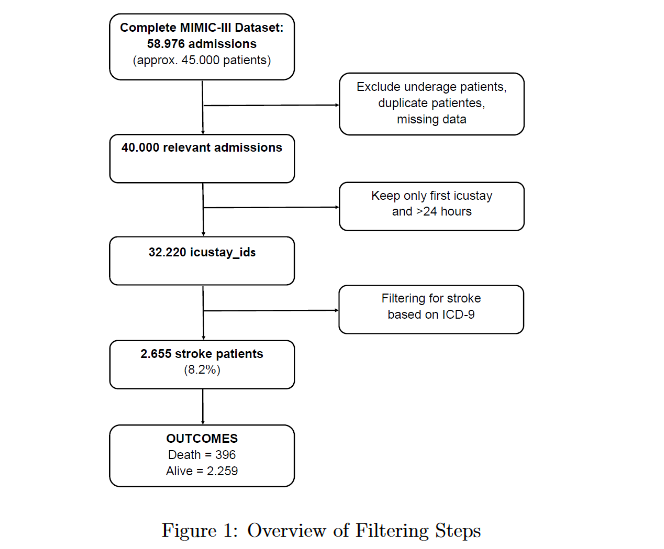
\includegraphics[width=0.7\linewidth]{screenshot001}
		\caption{}
		\label{fig:screenshot001}
	\end{figure}
	\subsubsection{Umgang mit Fehlenden Daten}
	%TODO Diagramm mit fehlenden Daten einfügen
	Die fehlende Uhrzeit in der Zeitreihe mit stündlichen Daten ergibt insgesamt sechs Monate fehlender Daten in 2020. 
	\begin {table} [ht]%TODO Tabelle hübsch machen
	\label{tab:fehlende-tage} 
	\centering
		\begin{tabular}{|l|l|}
			\hline
			2020-01-31  & 31\\
			2020-02-29  & 29\\
			2020-03-31  & 31\\
			2020-04-30  & 30\\
			2020-05-31  & 31\\
			2020-06-30  & 30\\
			\hline
		\end{tabular}
		\caption {Should be a caption} %TODO
	\end {table}
	%TODO Umgang damit, dass so eine große Lücke ist
	\begin{figure}
		\centering
		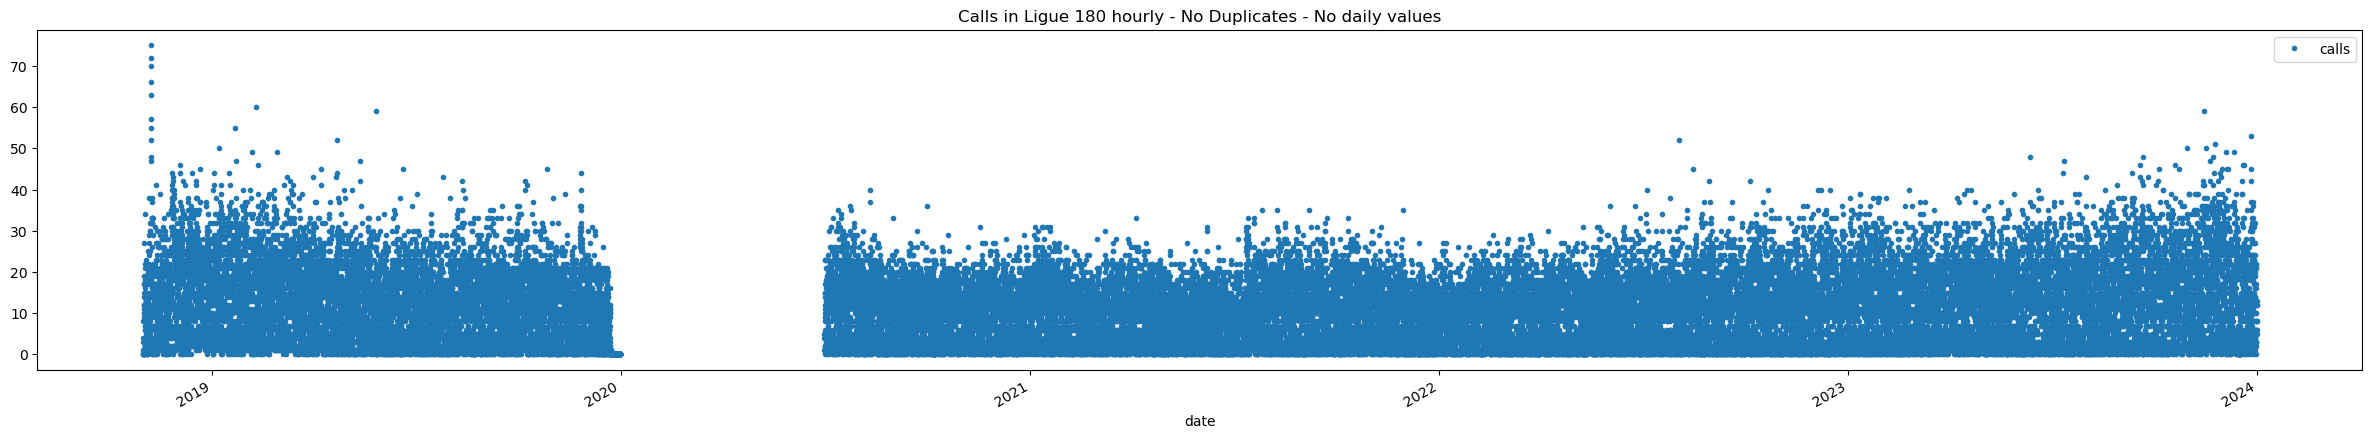
\includegraphics[width=1\linewidth]{screenshot003}
		\caption{}
		\label{fig:screenshot003}
	\end{figure}
	
	Umgang in df\_daily:\\
	- Nullwerte für df\_daily sind 1,5 Monate in März 2014 und 8 Tage im \begin{figure}
		\centering
		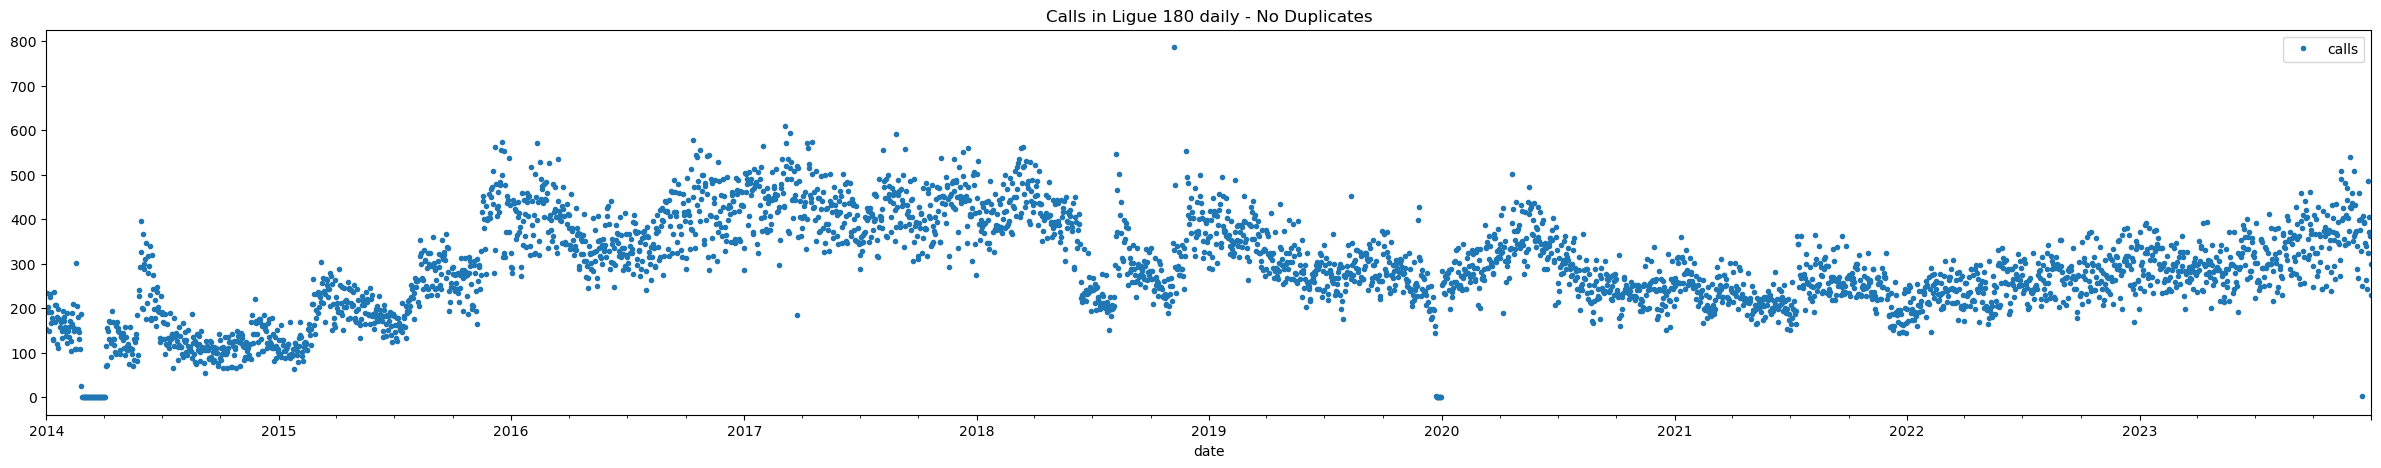
\includegraphics[width=1\linewidth]{screenshot002}
		\caption{}
		\label{fig:screenshot002}
	\end{figure}
	Dezember 2019
	Nullwerte für märz 2019: Daten sind für den Monat vorhanden im Balanco 2019, warum diese Daten nicht in der Statistik sind ist nicht klar.
	Dezember ist auffällig weil es vom 24. bis 31. ist: einerseits Vermutung, dass da besonders viele Anrufe sind wegen Feiertage, Alkohol, Familienstreit aka nicht null. Deswegen kann ich mir nicht vorstellen, dass die zu hatten. Vielleicht haben sie aber keine Anzeigen aufgenommen, aber dann funktionieren auch die Schutzmaßnahmen nicht. 
	
	%TODO Recherche warum an diesen Tagen keine Anrufe waren und umliegende DAten anschauen
	\subsubsection{Clusteranalyse von Nutzungsgruppen}
	%TODO Beschreiben der Vorbereitung des Datensatzes bei H2
	\subsection{Feature Vorbereitung}
	Der Datensatz enthält 62 verschiedene Kategorien. \\
	- Zusammenführen der Datensätze, inwieweit möglich? \\
	- Tabelle mit verschiedenen Kategorien \\
	- Tabelle mit Menge der Values\\
	- Zusammenführung von Values - Übersicht\\
	- Zusammenhangsgrafik der Kategorien (die vom Tablet) \\
	- Anhang mit Kategorien und Werten\\
	\subsubsection{H1}
	- Daten die zwischen leeren Tagen Monaten liegen bei df\_hourly?\\
	- hinzufügen der Ferientage: Ferientage eingetragen, mit Differenz: -1 bedeutet einen Tag nach Feiertag und +1 einen Tag vor Feiertag
	- Ergebnisse sind \ref{tab:differenz-zu-feiertagen}
	\begin {table} [ht]%TODO Tabelle hübsch machen
	\label{tab:differenz-zu-feiertagen} 
	\centering
	\begin{tabular}{|l|l|}
		\hline
		1    & 90\\
		2    & 90\\
		0    & 98\\
		-1    & 88\\
		3    & 88\\
		... & ~ \\
		-56    & 10 \\
		-57     & 10\\
		-58     & 10\\
		-59     & 10\\
		-60     & 10 \\  
		\hline
	\end{tabular}
	\caption {days\_to\_holiday for daily dataset from 2014 to 2023} %TODO
	\end {table}
	- Das gleiche für df\_daily gemacht
	\subsection{Feature Auswahl}
	\subsubsection{H1}
	-> Nullwerte für df\_hourly schon gezeigt\\
	
	- Daraus Schlussfolgerung welche Daten gewählt werden\\
	- Tabelle mit Nullwerten\\	
	- 
	\section{Künstliche Intelligenz} %Dieses Kapitel wird wahrscehinlich nirgends sinnvoll reinpassen
	\label{sec:ki}
	Die Künstliche Intelligenz ist das mit vielen verschiedenen Hoffnungen verbundene zukunftsweisendste Forschungfeld der Gegenwart. Die großen Hoffnungen und Erwartungen begründen sich auch in den vielfältigen Ansätzen und Techniken, die in den Bereich der künstlichen Intelligenz fallen \cite[S. 2]{Ege.2021b}. So gehört zum Bereich künstliche Intelligenz laut \cite[S. 2]{Ege.2021b}:
	\begin{itemize} \itemsep0pt
		\item die Logik, z.B. Aussagenlogik, Prädikatenlogik, Entscheidbarkeit,
		\item unsicheres Wissen und Schlussfolgerungen, z.B. Bayessche Netze, Fuzzy-Logik,
		\item Suchstrategien, z.B. uninformierte Suche, heuristische Suche,
		\item Wissensrepräsentationen, z.B. Ontologien und Semantic Web,
		\item Machine Learning, z.B. neuronale Netze und Deep Learning in Kombination von supervised und unsupervised Learning und Reinforcement Learning,
		\item Natural Language Processing,
		\item Computervision,
		\item Robotik.
	\end{itemize}	
	Bei den verschiedenen Ansätzen wird zwischen symbolischen und nicht-symbolischen unterschieden. Symbolische Ansätze bezeichnen Techniken und Ansätze des Maschinellen Lernens bei denen die Merkmale und Zusammenhänge von Mustern expliziert und repräsentiert sind. Das Verhalten dieser Techniken ist nachvollziehbar, kalkulierbar und interpretierbar. Zu diesen Techniken gehören Entscheidungsbäume, Ontologien, das Semantic Web und Wissensgraphen \cite[S. 9]{Ege.2021b}. Nicht-symbolische Ansätze speichern Wissen implizit. Dieses Wissen muss anhand großer Datensätze trainiert werden. Die Ergebnisse der Wissensrepräsentationen sind deshalb unvorhersehbar und manchmal auch nicht nachvollziehbar \cite[S. 9]{Ege.2021b}
	
	\chapter{Explorative Datenanalyse}
	Im folgenden Kapitel wird Anhand der Methoden in \cite{Walker.2024} %TODO Quellen
	erforscht, in welchem Zusammenhang die Daten miteinander stehen. 
	\section{Datenmenge}
	Erste Fragen zu dem Datensatz aus \cite[S.77f.]{Walker.2024}.
	Die kleinste Einheit im Datensatz, also der unique identifier: hash
	Menge der Daten: Spalten x Reihe
	%TODO Tabelle mit Mengen
	Key categorical values and the frequencies of each value?
	%TODO Tabelle mit allen relevanten Variablen
	%TODO Tabelle mit Begründung warum andere Variablen nicht relevant sind
	Verteilung kontinuierlicher Variablen
	%TODO raussuchen
	%TODO Verteilung berechnen
	Zusammenhänge zwischen den einzelnen Variablen
	%TODO 
	Variablen mit Werten außerhalb des Erwartungsbereichs und fehlende Werte
	%TODO
	
	\section{Verständnis für Daten}
	"When working with time series, it is critical that you learn more about the data you are working with and how it relates to the problem you are attempting to solve. For example, when working with manufacturing or sales data, you cannot assume that an organization's working day is Monday to Friday or whether it uses the standard calendar year or fiscal year. You should also consider understanding any holiday schedule, annual shutdowns, and other matters related to the business operation." aus Atwan.2022 \textit{Time Series Analysis with Python Cookbook}.
	\section{Forecasting der Anrufquote}
	Anhand des Methodenbuchs \textit{Time Series Analysis and Forecasting} der Autoren \textsc{Montgomery, Jennings, Kulahci} 2015 \cite{Montgomery.2015} werden im folgenden die Schritte beschrieben, die für eine Analyse im Bereich Forecasting benötigt werden.\\
	\subsection{Data Collection and Cleaning}
	Zu Beginn ist es wichtig die vorhandenen verfügbaren Daten auf ihre Nützlichkeit zu prüfen. Es können Werte fehlen, Daten verfälscht sein oder jegliches anderes Datenproblem auftreten. Hier muss festgehalten werden, welche Daten weshalb genutzt werden \cite[14]{Montgomery.2015}. \\
	Außerdem sollten die Daten bestimmten Gütekriterien entsprechen, laut \cite[17]{Montgomery.2015} sind diese \textit{ \glqq accuracy, timeliness, completeness, reprensatativeness, and consistency\footnote{Übersetzung:\textit{\glqq Genauigkeit, Aktualität, Vollständigkeit, Repräsentativität und Konsistenz.\grqq }}.\grqq} Im folgenden Abschnitt wird geprüft, ob die Daten diese Kriterien erfüllen.
	\subsubsection{Accuracy}
	Die Genauigkeit misst die Nähe der abgebildeten Daten zu den Daten in der Realität. 
	\subsubsection{Timeliness}
	Die Daten sollten bei einem Forecasting in die Zukunft so aktuell wie möglich gehalten werden, um eine genaue Vorhersage sicherzustellen. 
	\subsubsection{Completeness}
	Die Vollständigkeit verlangt vom Datensatz, dass es keine Ausreißer und fehlenden Werte gibt. 
	\subsubsection{Representativeness}
	Die vorhandenen Daten sollten für die Fragestellung geeignet sein, beispielsweise ist es nicht sinnvoll, die Daten der Hotline zu verwenden, um im allgemeinen Vorherzusagen, wann Gewalt gegen Frauen in Brasilien geschieht.
	\subsubsection{Consistency}
	Dieses Gütekriterium verlangt Konsistenz innerhalb der Zeitreihe, nicht nur inhaltlich sondern auch Formate und die Bedeutung von Kategorien und die Struktur des Datensatzes.
	
	\subsection{Data Analysis}
	Im Vorbereitungsschritt der Datenanalyse werden ist es wichtig die Zeitreihe auch visuell aufzubereiten. Dadurch können saisonale Muster oder Trends erkannt werden\cite[14f.]{Montgomery.2015}. 
	Im Fall der vorliegenden Daten ergeben  sich starke Differenzen in den Aufzeichnungen zwischen den Jahren 2014 und 2023.\\
	%TODO Grafik mit Zeitreihe
	%*Analyse welchen Zeitraum man weshalb genommen hat
	Ein weiterer Teil der vorbereitenden Analyse sind die Berechnung der statistischen Kennzahlen, wie Sample Mean, Standardabweichung, Perzentile und Autokorrelationen.\\ %siehe Chapter 2 in Montgomery.2015
	Ebenfalls ist es sinnvoll potenzielle Ausreißer festzuhalten, um sie später auf ihre Passbarkeit zu prüfen. Diese Vorbereitungen sind wichtig um ein Gefühl für die Daten zu bekommen und die Ergebnisse besser einordnen zu können \cite[15]{Montgomery.2015}.\\
	\subsection{Modellvergleich}
	
	\chapter{Methodik} %TODO jemand hat das Unterteilt in Entwurf, Implementierung und Evaluierung
	\section{Defining Modelling Objective}
	\section{Datenvorverarbeitung}
	In dem Leitfaden \textit{Data Preparartion for Machine Learning} beschreibt \cite{Brownlee.2020} die Datenvorbereitung als elementaren Bestandteil der Analyse. Er argumentiert, dass die Verarbeitungsalgorithmen seit Jahren bekannt sind, jedoch die evaluierten Datensätze die Innovation mitbringen, weswegen diese besonders gut verarbeitbar sein sollten \cite[14]{Brownlee.2020}. Demnach ist das,  was die Qualität der Studien ausmacht, nicht der ausgewählte Algorithmus, sondern die Verarbeitung der Daten von Rohdaten zu Daten für die maschinelle Verarbeitung \cite[9]{Brownlee.2020}. Dabei muss herausgefunden werden, wie die zugrunde liegende Struktur des Datensatz bestmöglich herausgearbeitet werden kann \cite[8]{Brownlee.2020}. Das ist abhängig davon, welcher Algorithmus verwendet werden soll, um das Modell zu erstellen \cite[12]{Brownlee.2020}. 
	\subsection{Vorverarbeitungsschritte}
	Je nach Algorithmus können irrelevante oder korrelierende Daten die Vorhersage des Modells verschlechtern. Die Wahl der Vorverarbeitung hängt zudem auch von dem vorliegenden Datensatz ab. Im Prozess des Feature Engineerings werden entscheidende Features, die das Design des Models mitbestimmen herausgearbeitet \cite[12]{Brownlee.2020}.\\	
	Bei der Wahl der Vorverarbeitungsschritte können zwei Es gibt den Ansatz durch das Modellieren herauszufinden, welche Schritte in der Datenvorverarbeitung notwendig sind. So können die Zusammenhänge der Daten beim Erstellen des Modells herausgearbeitet werden \cite[13]{Brownlee.2020}. Auf der anderen Seite gibt es die Möglichkeit, sich für jede Datenzeile zu überlegen, wie diese Aussehen müsste, um bestmöglich deren Charakter herauszuarbeiten \cite[13]{Brownlee.2020}. Der Autor plädiert dafür, eine Balance zwischen den beiden Ansätzen zu finden, da beide Ansätze mächtig seien und zu einer Ausarbeitung der zugrunde liegenden Struktur beitrügen \cite[13]{Brownlee.2020}.\\
	Entscheidend ist laut \cite[25ff.]{Brownlee.2020} ebenso die Reihenfolge der Vorverarbeitungsschritte. Der Autor benennt folgende Schritte als gängige Praxis: 
	\begin{itemize} \itemsep0pt
		\item Prepare Dataset
		\item Split Data
		\item Evaluate Model.
	\end{itemize}
	Diese Reihenfolge sieht er kritisch, da sie zu data leakage\footnote{Data leakage bedeutet, dass das Model Informationen erhält, die zu einem Vorteil für eine bessere Modellierung werden. Das können Testdaten sein, die den Trainingsdaten zur Verfügung stehen oder wenn Informationen aus der Zukunft der Vergagenheit zur Verfügung stehen \cite[93]{Zheng.2018}.} führen kann und somit das Modell beeinflussen kann \cite[26]{Brownlee.2020}. Ein Beispiel für data leakage findet sich in der Normalisierung einer Variable in der Skala von 0 bis 1. Dafür muss Minimum und Maximum aller Variablen identifiziert werden und somit erhält das Model Informationen über die globale Verteilung und somit über die Testdaten. Bei vielen Methoden, um Daten zu normalisieren und leere Felder zu füllen greift dieser Mechanismus.\\
	Aus diesem Grund plädiert \cite{Brownlee.2020} für diese Schritte, um die Daten vorzuverarbeiten:
	\begin{itemize} \itemsep0pt
		\item Split Data
		\item Fit data preparation on Training Dataset
		\item Apply Data Preparation to Train and Test Datasets
		\item Evaluate Models.
	\end{itemize}
	Nicht nur die Vorbereitung der Daten sollte nur mit dem Trainingsdatensatz erfolgen; dieser Ansatz sollte die gesamte Modellierung umfassen, wie Feature Selection, Feature Engineering und  Dimensionality Reduction \cite[27]{Brownlee.2020}.\\
	Diese Vorannahmen führen dazu, dass der erste Schritt der Vorverarbeitung die Einteilung in Test- und Trainingsdaten ist.
	\subsubsection{Unterteilung der Daten in Trainings und Testdaten}
	Einladen der Daten als Panda-Dataframe\\
	Verbinden der Jahre 2021 bis 2023\\
	Nutzen der Methode train\_test\_split von sklearn.model\_selection\\
	\subsubsection{Grundlagen der Datenbereinigung} 
	
	
	\section{Auswertungsmethoden}
	\chapter{Results}
	\section{Structure Learning}
	\section{Auswertungskriterien}
	\chapter{Discussion}
	\section{Preparation of Data}
	\section{Structure Learning}
	\section{Auswertungskriterien}	
	\chapter{Limitations}	
	\chapter{Conclusion}
	
	\newpage
	\clearpage
	
	
	
	\chapter*{Bibliography}
	\addcontentsline{toc}{section}{Bibliography}
	\bibliographystyle{abbrvdin}
	%\renewcommand{\refname}{}
	\bibliography{Literatur}
	
	\newpage
	
	
	\appendix %Anhang
	\pagestyle{empty}
	\pagenumbering{Roman}
	\setcounter{page}{1}
	\chapter{Appendix}
	
	\chapter*{Erklärung der Urheberschaft}
	
	Ich erkläre hiermit an Eides statt, dass ich die vorliegende Arbeit
	ohne Hilfe Dritter und ohne Benutzung anderer als der angegebenen
	Hilfsmittel angefertigt habe; die aus fremden Quellen direkt oder
	indirekt übernommenen Gedanken sind als solche kenntlich gemacht. Die
	Arbeit wurde bisher in gleicher oder ähnlicher Form in keiner anderen
	Prüfungsbehörde vorgelegt und auch noch nicht veröffentlicht.
	
	\vspace{4cm}
	
	\hspace{2cm} Ort, Datum \hfill Unterschrift \hspace{2cm}
	
	
	
\end{document}